% Change to 'masters' to produces the masters thesis preliminary pages
\documentclass[oneside,phd,etd]{WSUclass}

\usepackage{import}
\usepackage{tabularx}
%\usepackage{cleveref}
\usepackage{booktabs} %for table divider lines
\usepackage{array}
% metadata contains title page, signature page, acknowledgment and abstract texts
\usepackage{metadata}
\usepackage{caption}
\captionsetup[table]{labelfont={sc},singlelinecheck=false,skip=25pt,belowskip=8pt}

\usepackage{xstring}

% Pacakges used
\usepackage[utf8]{inputenc} % Remove warning on ascii conversion
\usepackage[T1]{fontenc} % Remove warning on ascii conversion
\usepackage[citestyle=IEEE,natbib=true,backend=biber,style=numeric-comp]{biblatex}
\addbibresource{BibFile.bib}

\usepackage{hyperref}
\usepackage{cleveref}
% Make chapter numbers into string words 1 -> ONE
\usepackage{fmtcount}
\usepackage{amsmath}
\usepackage[]{standalone}

\makeatletter
\renewcommand{\@makechapterhead}[1]{\vspace *{40\p@ }{\parindent \z@ 
\raggedright \normalfont \ifnum \c@secnumdepth >\m@ne \Huge \bfseries 
\@chapapp \space \Numberstring{chapter} \vskip 10\p@ \fi #1\par \nobreak \vskip 30\p@ }}
\makeatother


\begin{document}
\let\oldcref\cref
\renewcommand{\cref}[1]{\Cref*{#1}}
\hypersetup{breaklinks=true}

% Start page counting in roman numerals
\frontmatter

% This command makes the formal preliminary pages.
% You can comment it out during the drafting process if you want to save paper.
\makepreliminarypages
\clearpage

\doublespace
% Make the table of contents.
\tableofcontents
\thispagestyle{plain}

% Make the list of tables
\mylistoftables
\thispagestyle{plain}

% Make the list of figures
\mylistoffigures
\thispagestyle{plain}

% This page is OPTIONAL. To remove, comment out and \dedicationpage in diss.tex
\dedicationpage
\clearemptydoublepage

% Start regular page counting at page 1
\mainmatter

% OK. Everything is set up. Type your thesis here.
%include does NOT work for relative paths going UP the directory, so am using input.
\addchapheadtotoc
\chapter{SOME FORMATTING EXAMPLES}
\section{Chapter one tittle section}
TBA
\subsection{Another subsection of section - citations}
Example of citation \cite{altschul1997gapped}. TBA


Example of multiple citations \cite{altschul1997gapped, baker2007novel}.TBA.
\subsubsection{Subsubsection of section - italic text}
TBA.

\chapter{LINKS}
\section{Chapter one tittle section - links examples}
TBA.
\subsection{Subsection title - more links examples}.
Another example of hyperlink \href{http://www.wikibooks.org}{Wikibooks home}.
\chapter{FIGURES AND TABLES}
\section{Examples of a figure}

Example of a figure.
\begin{figure}[ht!]
\begin{center}
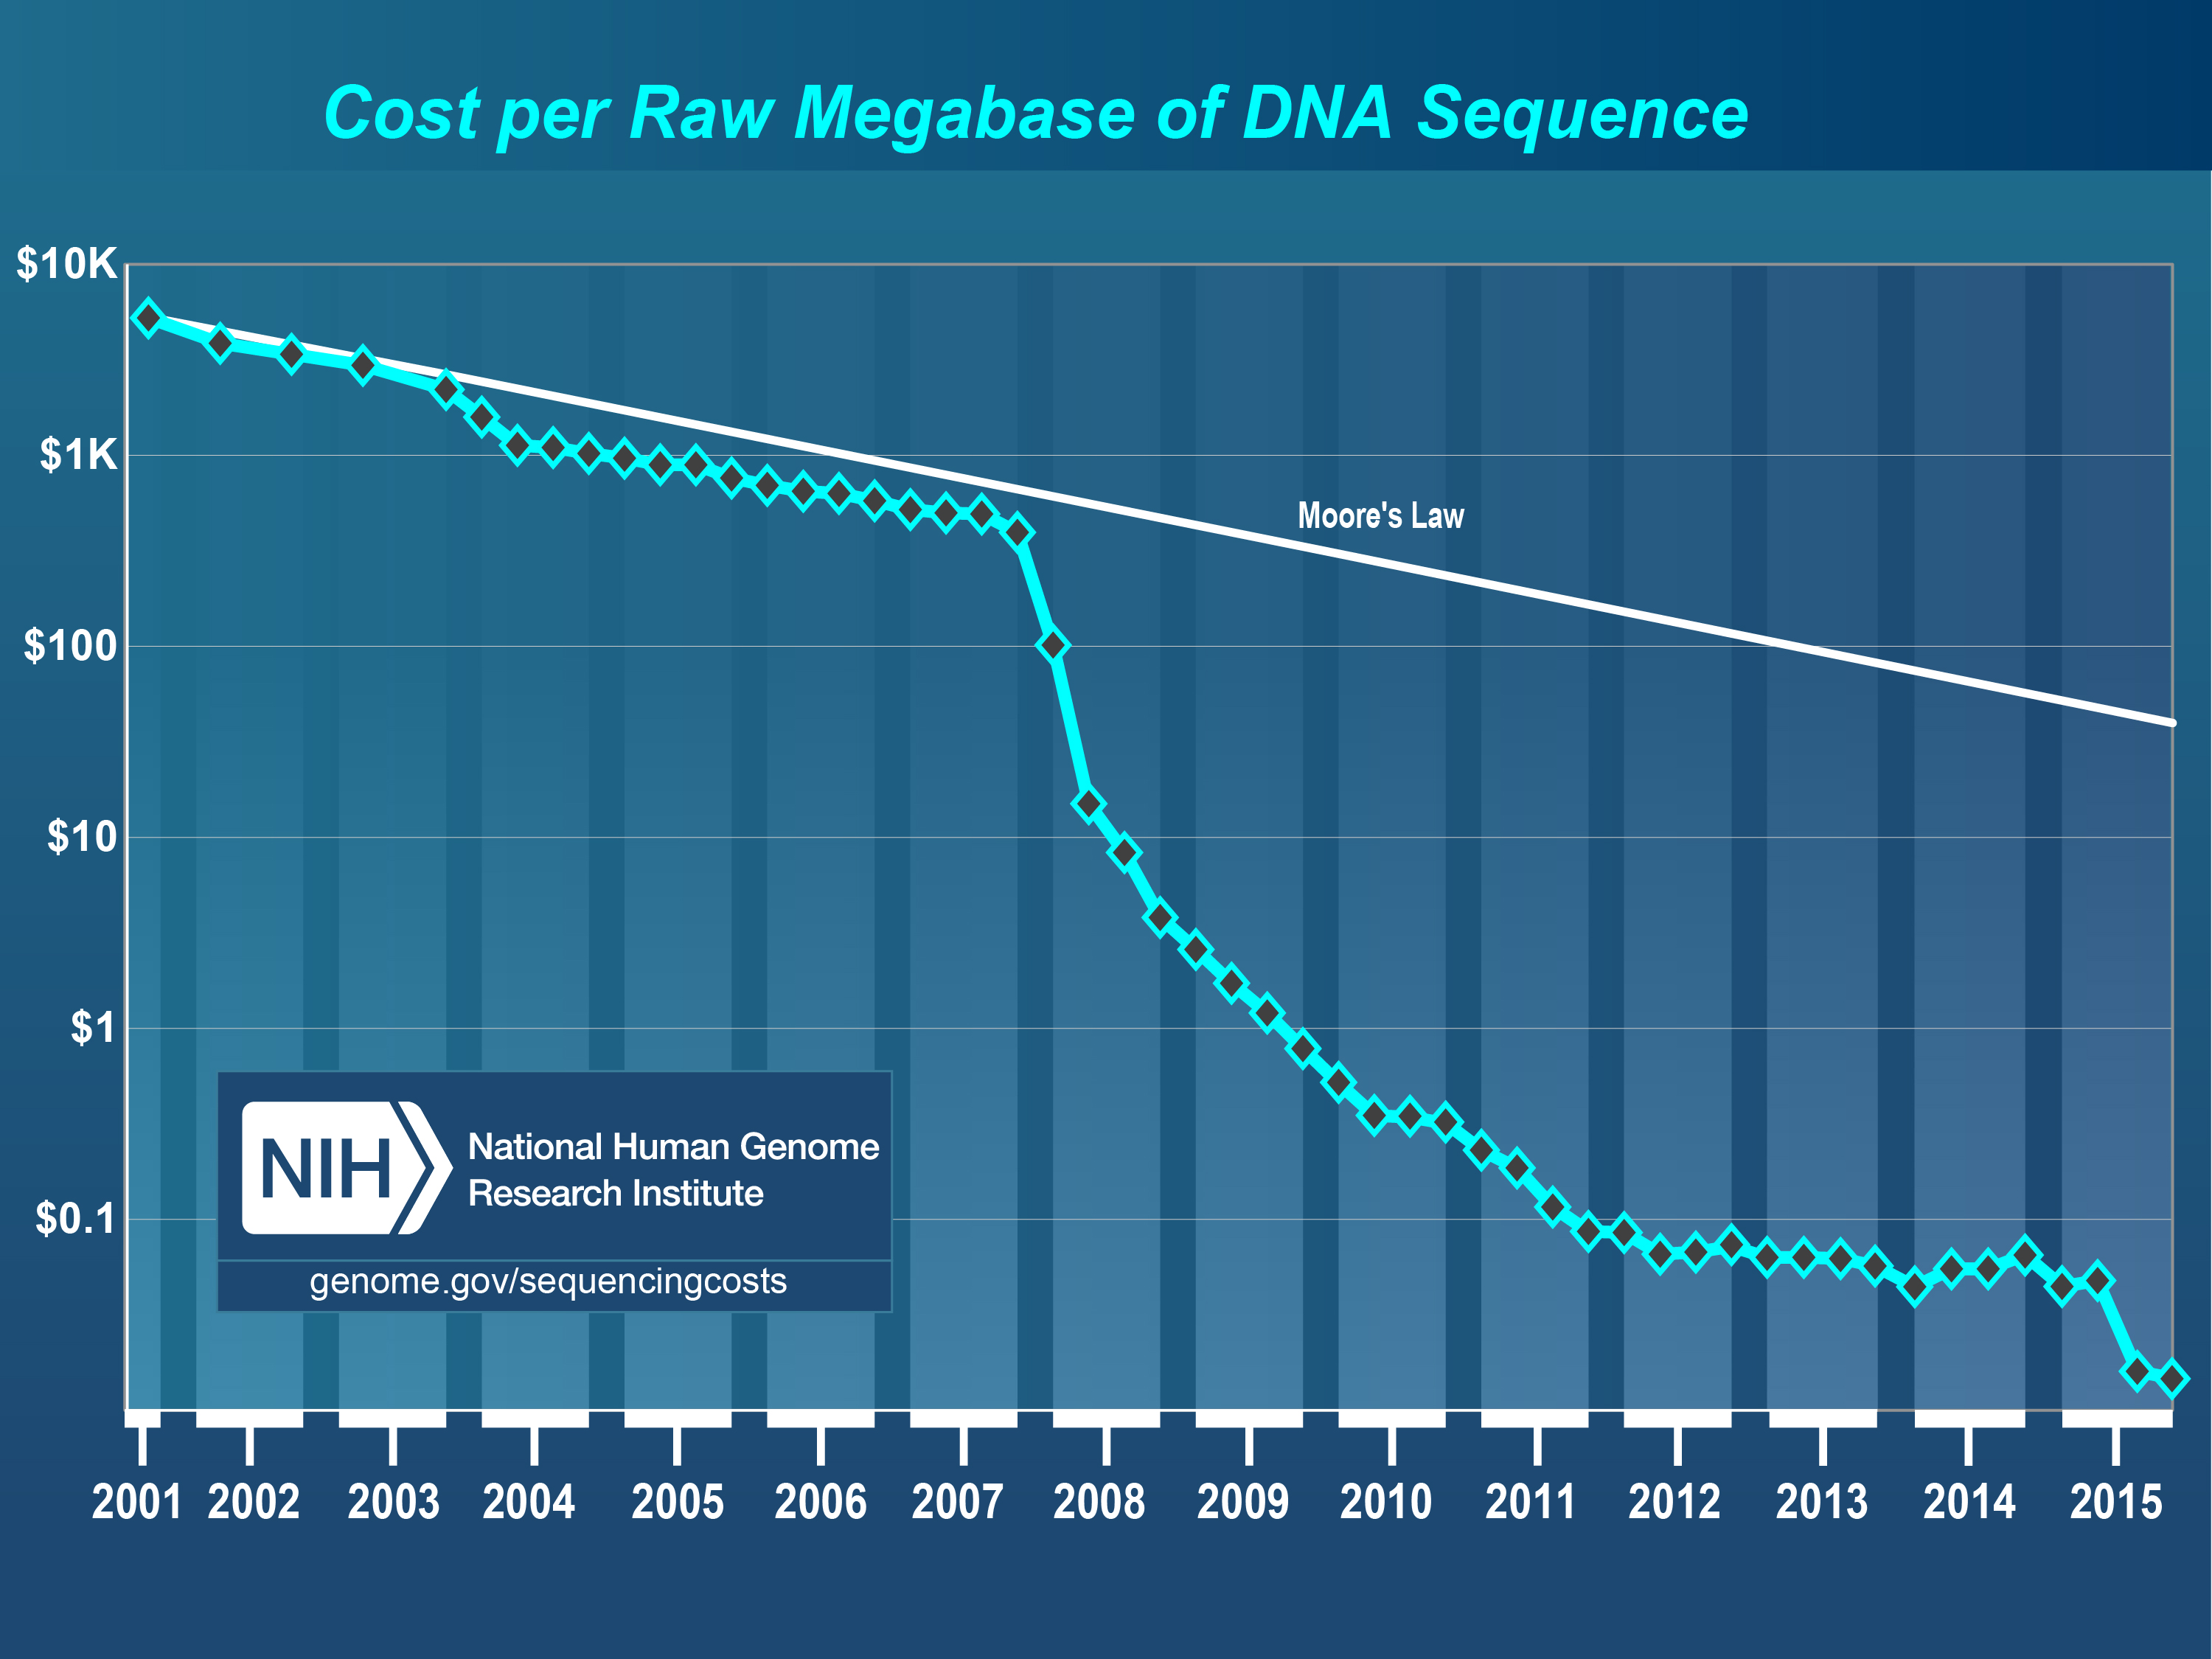
\includegraphics[scale=0.5]{../images/costperMb2015_4.jpg}
\end{center}
\caption[hehe]{Cost per raw megabase of DNA sequence from 2001 to 2015. Straight line - Moore's Law, blue curve - cost in US dollars, Y-axis scale is logarithmic. Graph reproduced from \cite{wetterstrand2016}}
%Source:
\label{fig_dna_cost}
\end{figure}

Example of reference to a figure in the text (Fig.~\ref{fig_dna_cost}).




% Bibliography
\begingroup
    \setlength\bibitemsep{10pt}
    \linespread{1}\selectfont
    \printbibliography[title=REFERENCES]
\endgroup
\addcontentsline{toc}{part}{REFERENCES}

% Appendices
\appendix

%%%%%%%%%% DON'T DELETE THIS, REVERTS NUMBERING BACK %%%%%%%%%%%%%
\makeatletter
\renewcommand{\@makechapterhead}[1]{\vspace *{-10\p@ }{\parindent \z@ 
\raggedright \normalfont \ifnum \c@secnumdepth >\m@ne \Huge \bfseries 
\@chapapp \space \thechapter \vskip 10\p@ \fi #1\par \nobreak \vskip 30\p@ }}
\makeatother
%%%%%%%%%% DON'T DELETE THIS, REVERTS NUMBERING BACK %%%%%%%%%%%%%

\chapter{Example of a table}
%\section{Example of a table}
Example of a table and here is the reference to Table \ref{tab:bfm1}. Tables in, my opinion, are the hardest thing to make.

%\section{Branch Flow Model: Relaxations and Convexification}
\chapter{Branch Flow Model: Relaxations and Convexification}
\begin{table}[!h]
	\caption{Table describing the Branch Flow Model equations.}
	\label{tab:bfm1}
	\centering
	\hspace*{-2cm}
	%\documentclass{standalone}
%\usepackage{booktabs}

%\begin{document}
	\small
	\begin{tabular}{clccc} 
		\toprule
		Equation \# & Equation & Unknowns & Knowns & No. of Equations \\
		\midrule
		13 & $p_j = \Sigma P_{jk} + \Sigma (P_{ij} - r_{ij}l_{ij}) + g_jv_j$ & \begin{tabular}{c}
			$1 \times p_0$ \\
			$m \times P_{ij}$ \\
			$m \times l_{ij}$ \\
			$n \times v_j$
		\end{tabular} &
		\begin{tabular}{c}
			$n \times p_j$ \\
			$m \times r_{ij}$ \\
			$(n+1) \times g_{j}$ \\
			$1 \times v_0$
		\end{tabular} & $(n+1)$ \\
		\midrule
		14 & $q_j = \Sigma Q_{jk} + \Sigma (Q_{ij} - x_{ij}l_{ij}) + b_jv_j$ & \begin{tabular}{c}
			$1 \times q_0$ \\
			$m \times Q_{ij}$ \\
			$m \times l_{ij}$ \\
			$n \times v_j$
		\end{tabular} &
		\begin{tabular}{c}
			$n \times q_j$ \\
			$m \times x_{ij}$ \\
			$(n+1) \times b_{j}$ \\
			$1 \times v_0$
		\end{tabular} & $(n+1)$ \\
		\midrule
		15 & $v_j = v_{i} +  (r_{ij}^2 + x_{ij}^2)l_{ij} - 2(r_{ij}P_{ij} + x_{ij}Q_{ij})$ & \begin{tabular}{c}
			$m \times P_{ij}$ \\
			$m \times Q_{ij}$ \\
			$m \times l_{ij}$ \\
			$n \times v_j$
		\end{tabular} &
		\begin{tabular}{c}
			$b \times r_{ij}$ \\
			$m \times x_{ij}$ \\
			$1 \times v_0$
		\end{tabular} & $m$ \\
		\midrule
		16 & $l_{ij} = \frac{P_{ij}^2 + Q_{ij}^2}{v_j}$ & \begin{tabular}{c}
			$m \times P_{ij}$ \\
			$m \times Q_{ij}$ \\
			$m \times l_{ij}$ \\
			$n \times v_j$
		\end{tabular} &
		\begin{tabular}{c}
			$1 \times v_0$
		\end{tabular} & $m$ \\
		\midrule
		13 to 16 & {} & \begin{tabular}{c}
			$1 \times p_0$ \\
			$1 \times q_0$ \\
			$m \times P_{ij}$ \\
			$m \times Q_{ij}$ \\
			$m \times l_{ij}$ \\
			$n \times v_j$
		\end{tabular} &
		\begin{tabular}{c}
			$n \times p_j$ \\
			$n \times q_j$ \\
			$m \times r_{ij}$ \\
			$m \times x_{ij}$ \\
			$(n+1) \times g_j$ \\
			$(n+1) \times b_{j}$ \\
			$1 \times v_0$
		\end{tabular} & $2(n+1+m)$ \\
		\midrule
		{} & {} & $2(n+1+m)$ & $4n+2m+3$ & $2(n+1+m)$ \\
		\bottomrule
	\end{tabular}
%\end{document}

\end{table}

\chapter{Abstracts: Optimization-based Methods for solving MP-OPF}
\lipsum

\chapter{Abstracts: Dynamic Programming Methods for solving MP-OPF}
\lipsum

\end{document}
